\documentclass[11pt]{article}
\renewcommand{\baselinestretch}{1.8}
\usepackage{textcomp}
\usepackage{fontenc}
\usepackage{graphicx}
\usepackage{caption} % for Fig. captions
\usepackage{gensymb} % for \degree
\usepackage{placeins} % for \images
\usepackage[margin=1in]{geometry} % to set margins
\usepackage{setspace}
\usepackage{lineno}
%\usepackage{cite}
\usepackage{amssymb} % for math symbols
\usepackage{amsmath} % for aligning equations
\usepackage{natbib}
\bibliographystyle{..//..//sub_projs/refs/styles/besjournals.bst}
\usepackage{xr-hyper}
\externaldocument{diffsens_SUPP}



\linenumbers


\title{Differences in flower and leaf bud responses to the environment drive shifts in spring phenological sequences of temperate woody plants}\\

\date{}
\author{D.M. Buonaiuto $^{1,2,a}$, E.M. Wolkovich$^{3}$}

\begin{document}
\maketitle

Some ideas for journals: Nature Plants, Journal of Ecology, Plant, Cell and Environment. Currently about 4,000 words. (3,000 without methods). Intro is about 1,100. 34 refs, but missing a few needed. \\
\section*{Abstract} %EMWOct2 -- someday need a better opening sentence, it's the right point, just not the best phrasing, either need a better term that 'fitness character' or something like ... by structuring the timing of growth versus reproduction, the temporal relationship between vegetative and reproductive phenology, shapes fitness for deciduous woody species... 
The temporal relationship between vegetative and reproductive phenology is an important fitness character for deciduous woody plants. These flower-leaf sequences (FLSs) appear to be shifting with climate change, but predicting the impacts of these shifts requires an improved understanding of how the enviroment dictates FLS patterns. We compared the phenological responses of flower and leaf buds to varying temperature and light conditions for a suite of temperate woody species to test two competing hypotheses regarding underlying physiology of FLS variation. We found that flower and leaf buds respond with differential sensitivity environmental cues, with differences in their response to chilling being the dominent driver of FLS variation. These findings suggest that climate change can generate substantial FLS shifts, which is likely to affect population and community structure in the coming decades. %131 words so probably could add a sentence or 2
 %EMWOct2 -- abstract doesn't sound as interesting and important as the paper does 

\section*{Introduction}
\noindent One of the most widely documented biological effects of anthropogenic climate change are shifts in phenology, the timing of life cycle events, in plants \citep{Parmesan2003,Menzel2006,Cleland2007}. While phenology is generally advancing with climate change, the strength of these phenological shifts can vary substantially among specific phenological phases \citep{Augspurger:2020aa}. These differences alter the timing of phases relative to each other, changing the duration of inter-phase periods that make up phenological sequences \citep{Ettinger2018}. As a major driver of plant fitness that impacts plant life history, resource allocation, demography and ecosystem processes \citep{Post:2008aa}, shifting phenological sequences with climate change will likely impact many of these processes. However the effects these shifts depend both on the direction (whether distinct phases are shifting closer together or farther apart) and magnitude (how much they are shifting relative to each other).\\ %EMWAug6: Nice! %EMWSep21: Still very nice, but can we clean up the flow of the last three sentences? I think part of the problem is that we say 'phenological sequences' a few too many times, but take a look. I can work on it too next draft.  %EMWOct2 -- these last two sentences are way more exciting than the abstract, for example.

\noindent Among deciduous woody plants, the relative timing of flower and leaf phenology, or flower-leaf sequences (FLSs), may be particularly consequential to fitness in temperate regions where flowering prior to leaf development is common \citep{Rathcke_1985,Gougherty2018}. Flowering before leaf development may be a critical adaptation for pollination efficiency in wind-pollinated taxa by eliminating pollen interception by the forest canopy \citep{Whitehead1969}. In insect-pollinated taxa, flowering-first may increase the visibility of flowers to pollinators \citep{Janzen1967,Savage2019} or alleviate hydraulic demand in dry conditions \citep{Gougherty2018, Franklin2016}.\\ %Long-term phenological observations over the last several decades indicate that, like other phenological sequences, FLSs are shifting due to anthropogenic climate change \citep{Buonaiuto2020} suggesting that some of the critical functions of FLSs may become compromised. However, observed FLS shifts vary among species, which may put some species at greater risk while benefiting others \citep{Buonaiuto2020}.\\  %EMWAug6: May need to inject a clause in the first few sentences of this paragraph to help readers along ...  maybe change "Long-term phenological observations over the last several decades indicate that, like other phenological sequences, FLSs are shifting due to anthropogenic climate change \citep{Buonaiuto2020} suggesting that some of the critical functions of FLSs may become compromised." to 

\noindent Long-term phenological observations over the last several decades indicate that, like other phenological sequences, FLSs are shifting due to anthropogenic climate change \citep{Buonaiuto2020}. For several species, the time between flowering and leafing appears to be increasing, but the strength of this trend varies among species and the direction of FLS shifts are not consistent across populations \citep{Buonaiuto2020}. These changes could affect the important functions of FLSs, potentially putting some species at greater risk for fitness declines while benefiting others.\\ %EMWSep21: greater risk of what? (or rephrase)
%EMWSep21: Ah, okay -- you need a tighter transition between the above and below paragraph. You either need to set up pollination as being a big part of FLS above or introduce it here... you jump into it a little too much. 

\noindent Wind-pollinated species with decreasing FLS interphases with climate change may experience increased pollen limitation as more pollen is intercepted by vegetative structures and flowers are obscured by developing leaves. Conversely, pollination efficiency could improve for species with lengthening FLS interphases (direction). A change in the FLS interphase of just a few days would likely have little impact on these processes, but if shifts were on the order of weeks, the impact on the pollination biology of a species could be highly significant (magnitude).\\ %EMWOct2 -- good paragraph, just needs work at the end. Wonder if we should also mention it could affect models of plant dispersal or pollen models? Or link to at least some articles here on pollen models... 

\noindent Predicting the direction and magnitude of any FLS shifts requires identifying the underlying proximate mechanisms that drive responses to climate change among phenophases. %There is mounting evidence that plants respond more strongly to different environmental cues during different parts of their annual cycle. Cues use may vary among phenophases across the season because reliability of specific cues to indicate appropriate conditions changes over the season as well \citep{}. For example, woody plants rely more strongly on photoperiod as a cue for autumn phenological phases than for spring phases indicating that daylength is a more reliable cue for the cessation of growth than the start of growth\citep{}. However, this hypothesis does not explain different cue use among phenophases like spring flowering and leafing that occur close to each other in time under relatively similar conditions \citep{}.\\
Decades of research suggests that for woody plants in temperate regions, cool winter temperatures (chilling), warm spring temperatures (forcing) and day-length (photoperiod) are the primary drivers of both reproductive and vegetative phenology \citep{Forrest2010,Flynn2018}. However, observed FLS shifts indicate that there must be differences in how these cues influence phenological activity in floral and leaf buds \citep{Buonaiuto2020}. % but these differences have not been well characterized in wild species. 
Identifying these differences is a necessary step for predicting the direction, magnitude and---ultimately---fitness impacts of FLS shifts with climate change.\\ %EMWSep21: Need citation for "observed FLS shifts indicate that there must be differences ..." 
\subsection*{Hypotheses for climate drivers FLS variation} %need better title
\noindent Studies that have attempted to identify the differences between reproductive and vegetative phenology in woody plants (mostly focused on crop species) have yielded two common, yet competing, explanations:
%\noindent What we call the \textbf{precocity hierarchy hypothesis (PHH)} suggests that reproductive and vegetative buds respond similarly to most environmental cues, but have consistently different forcing requirements for the commencement of phenological activity \citep{Guo_2014,COSMULESCU:2020aa,Cosmulescu:2018aa}.  \\%EMWAug6: I would name the hypotheses after you introduce them ... some possible edits also:
% What we call the \textbf{precocity hierarchy hypothesis (PHH)} suggests that reproductive and vegetative buds respond similarly to most environmental cues, but have consistently different forcing requirements for the commencement of phenological activity --> 
\noindent One hypothesis suggests that reproductive and vegetative buds utilize the same underlying environmental cues, but have different threshold responses to forcing, with whichever bud type bursts later---leaves or flowers---having a higher threshold \citep{Guo2014,COSMULESCU:2020aa,Cosmulescu:2018aa}. Under this hypothesis, which we call the precocity hierarchy hypothesis (PHH), leaf and flower buds share the same suite of cues and develop similarly to non-forcing cues (i.e., chilling and photoperiod), but they differ in the thermal units required for budburst.\\ %EMWOct2 -- you need to do a sweep through the ms to decide what terms to use and make sure you define them -- thresholds, thermal sums etc.

\noindent In contrast, the alternative hypothesis suggests that flower and leaf buds differ in the strength of their phenological responses to the multiple environmental cues \citep{Citadin2001,Gariglio2006,Aslani2009,Mehlenbacher:1991aa}. Under this hypothesis, which we call the differential sensitivity hypothesis (DSH), each bud type relies more or less on certain cues, producing different and variable phenological patterns (even when leaf and flower buds are exposed to similar environmental conditions). This differential sensitivity has been observed for other phenological sequences in woody plants---for example the while temperature is the considered to be the primary driver of budburst phenology, budset is under strong photoperiodic control \citep{} which driver interannual variability in growing season length.\\ %EMWOct2 -- something bad happens halfway into this paragraph

%EMWOct2 -- I think a more logical next paragraph would start with: Under current field conditions, the PHH and DSH may produce similar phenological patterns, but experiments that disentangle all three cues should differentiate between the two. [Then I would just write out what is the figure, withOUT saying they come from simulations. We can discuss this next week... ]
\noindent Under current field conditions, the PHH and DSH may produce similar phenological patterns, and because of complex interactions between cues \citep{}, it can be difficult to neatly differentiate them. We simulated patterns of phenological sensitivity ($\Delta$ day of phenological event/ $\Delta$ environmental cue) to better understand the dynamics of cue responses for each of these underlying mechanisms (Fig. \ref{fig:simulations},Supplemental methods). From these simulations, we found that a key signature of the PHH is that the sensitivity to forcing of the second phase in the phenological sequence is 2x that of the first phase (Fig. \ref{fig:simulations} a.,b.).  We also found that interactions between the chilling response and forcing threshold requirements under the differential sensitivity framework can generate this signature of the PHH when secondary cues are at high levels (Fig. \ref{fig:simulations} c., chill x force interaction). It is therefore possible that the PHH is a special case of the DSH that occurs when the chilling and photoperiod requirements of both bud types have been met.\\
%EMWOct2 --Then I would have a short paragraph about the complexities -- this could include some of what you have above.

%EMWOct2 -- below two paragraphs are pretty good! I would just make sure that either above you more strongly explain why this matters (my comment about pollen and dispersal models) and here you might tie back to it. Spell out which types of species would do better or worse with climate change?
\noident While the hypotheses may be indistinguishable under current field conditions, they have different implications regarding the potential for FLS shifts with climate change. The PHH suggests that FLS variation is largely a product of climate variation during the interphase. If spring temperatures increase with climate change, the second phenophase of the FLS with be accelerated relative to the first and the FLS interphases will decrease, but given the relative auto-correlation of spring temperatures \citep{Di-Cecco:2018aa}, these shifts should be relatively muted. \\

\noindent The DSH suggests that with significant cue-use differences among bud types there will be strongly localized effects of climate change on FLSs. Shifts in FLS variation will depend on the direction and rate of change in cues at given locations and the species-specific differential sensitivity of reproductive and vegetative phenology to cue combinations. This hypothesis allows for larger magnitude shift in FLSs, and also suggests that the magnitude of shifts may be highly divergent both among species in a community, and among populations of the same species.\\%EMWSep21: I think we should add somewhere around here with a clear rationale/connection to the multi-species aspect of the study. (I removed one-clause mention of it from the cues paragraph as I think it's not needed there, but we do need to address it head-on and I think around here would likely work). You could weave this in with/set up why you did projections. It fits really nicely, but you're not making the connections for the reader! 
%DMB: I felt like we addressed species difference above, so I am just mentioning it here to transition

\noindent In this study we tested PHH and DSH hypotheses via a full factorial experiment manipulating chilling, focing and photoperiod cues for flower and leaf buds of 10 temperate shrub and tree species. We then leveraged these data to project how FLSs may shift with climate change and ....\\ % We then assessed species-level differences in FLS variability by observing phenological responses to changing environmental conditions for both flower and leaf buds. 
% "and identify avenues for further research." %EMWOct2 -- this line can fit in most studies ... Could you replace it with something more specific? This could be a spot to come back to why these hypotheses matter or such?

\section*{Methods}

\subsection*{Growth chamber study}
%EMWSep21: Add lat/long and dates should be day month year
\noindent We sampled all plant material from Harvard Forest in Petersham, MA (42.5314\degree N, 72.1900\degree W). On 25 October 2016, immediately after most plants in the area entered dormancy but before they could accumulate significant chilling in the field,  we collected branch cuttings from 7-13 individuals of 12 woody plant species (4-12 cutting per individual for a total of 48-56 per species). The species consisted of a mix of deciduous shrubs, understory and canopy trees commonly found in mesic hardwood forests of the eastern United States (see tab. \ref{tab:splist} for species list). We transported all cuttings to the Arnold Arboretum in Boston, MA where they were re-cut in water to prevent callousing and cavitation and placed in 500 ml Erlenmeyer flasks with distilled water.\\ 

\noindent We randomly assigned cuttings to a fully crossed set of eight experimental treatments; two levels of chilling (4 vs 8 weeks at 4\degree C), two levels of temperature (24\degree C:18\degree C (day/night) warm vs 18\degree:12\degree C (day/night) cool) and two levels of photoperiod (12 vs 8 hours). We alternated day/night temperature periodicity on a 12 hour schedule to reduce co-variation with photo-periodicity. We re-cut all twig and changed the water every 7-10 days and rotated all treatments between growth chambers every two weeks to minimize chamber effects. We made phenological observations every 2-3 days using a modified BBCH scale for woody plants \citep{Finn2007} for three months following release from chilling conditions. In this period we assess two phenological phases: budbreak (BBCH phase 07) %, leaf unfolding (BBCH phase 15) 
and first flower open (BBCH 60). At the conclusion of this period we assessed all individuals that did not undergo budbreak and excluded 56 dead individual twigs from our analyses. %EMWSep21: We probably should say how many this was to allay fears ... 

\subsection*{Data analysis}
\noindent To assess the sensitivity of each phase, we fit mixed-effect hierarchical models with chilling, forcing, photoperiod and all two-way interactions as the fixed effects and species as a grouping factor on both the slopes and the intercepts. We chose a Bayesian, hierarchical approach in order to identify systematic trends across species' responses while accounting for sample size, variance and the unique effect of each species. Two species \textit{Betula allegheniensis} and \textit{Acer saccharum} produced no flowers in our trial, so we excluded them from our analysis. In total, our analyses included 464 twigs from 10 species. \\

%emw8May2020: I think we can cut the below paragraph, as long as we specify the intercept condition in the captions (more useful to specify it there anyway); likewise use of dummy variables should be obvious when looking at model output and figures as long as clearly labeled (e.g., 4 hour difference) 
%\noindent Because we applied two levels for each environmental treatment in the experiment, we re-coded each treatment as 0/1 dummy variables to improve model performance, so model intercepts can be interpreted as the predicted phenological response when all treatments are at their lowest level. Given that true zeros for these treatment levels are unrealistic in nature, in addition to computational efficiency, this approach also allows for a realistic interpretation of model intercepts.\\  

\noident We modeled the effects of environmental parameters on flower opening and leaf budburst separately. We also fit a model with FLS interphase (day of budburst- day of flowering) as a response variable to compare these estimates with field observations.\\

The models we fit appear below:\\
%EMWOct2 -- is there an error term in this model?

$y_{[i]} \sim N(\alpha_{sp_{[i]}}+\beta_{forcing_{sp[i]}}+\beta_{chilling_{sp[i]}}+\beta_{photoperiod_{sp[i]}}+\beta_{forcing x chilling_{sp[i]}}+\beta_{forcing x photoperiod_{sp[i]}}+\beta_{chilling x photoperiod_{sp[i]}})$\\

Where $y_{[i]}$ is either the day of the experiment leaf budburst, day of first flower opening or FLS interphase length.  We modeled the $\alpha$ and each $\beta$ parameter at the species level using the formula:\\

$\alpha_{x_{sp}} $or $\beta_{x_{sp}} \sim N(\mu_x,\sigma^2_x)$\\

%EMWSep21: I think we may need to explain this hypothesis more to readers, especially as it matters to the results. Set up in intro?
\noindent To test our hypothesis that the PHH is a special case of the DSH that occurs when all secondary cues requirements are met, we re-ran our models on a subset of our data which included both levels of forcing treatment but only the high photoperiod and chilling treatment levels. This model included forcing as the only main effect but, like our main models written above, included species as a grouping factor on the model slope and intercept.\\ 

\noindent We fit all models using the R package ``brms" \citep{Burkner2018}. We ran each model on four chains with 4000 iterations with a 3000 iteration warm up for a total of 1000 sampling iterations. In all models we used weakly informative priors and increasing the priors 5-fold did not affect the model results.\\ %EMWSep21: n-eff? DMB Not sure how to report this %EMWOct2 -- check the budburst paper! or Flynn & Wolkovich ...

%EMWOct2 -- add in adding posteriors method, I think Cat reports this in her New Phyt false spring paper. 

\subsection*{Climate change predictions}
%EMWSep21: The below all reads very well!
\noindent To apply our model results to general climate change projections we chose our environmental treatments in this experiment to broadly reflect historic and future conditions at our sampling site. Our low forcing treatment approximated average spring temperature (March/April) at the site while our high temperature treatment reflects a 5 \degree C increase. Average field chilling (calculated from 15 Oct - 15 April, measured in Utah units) at Harvard Forest is 979.64, approximately 60\% of the difference between our low and high chilling treatment (Fig. \ref{tab:chillcomps}). Thus, our low chilling treatment represents a feasible estimate for a decrease in chilling with climate change and our high chilling treatment approximate reasonable increase. We should note that our low photoperiod treatment (8 hours of daylight) is well below the photoperiod experienced at Harvard Forest, but given that the photoperiod effects are expected to be small, we chose more extreme values in order to robustly estimate an effect (i.e., increasing statistical power). For this reason, our climate change projections for FLS variation are based on our high photoperiod treatment alone.\\

\noindent We used our flower and budburst models to project for each species in our study:\\
\begin{enumerate}
\item FLSs under average environmental conditions  (treatments: low forcing, ~6.5 weeks of chilling treatment)
\item FLS shifts with spring warming only (high forcing, ~6.5 weeks of chilling treatment)
\item FLS shifts with warming and increased chilling (high forcing, ~8 weeks of chilling treatment)
\item FLS shifts with warming and decreased chilling (high forcing, ~4 weeks of chilling treatment)

\end{enumerate}

\noindent To validate our predictions, we compared our FLS interphase model estimates of ``average" condition FLS interphases to long term phenological records from Harvard Forest \citep{OKeefe2015} for five species common to both datasets (Fig. \ref{fig:validate}), and found them to be comparable. Given the variable dynamics of shifts in environmental forcing and chilling with climate change over time and space, these projections should not be treated as absolute predictions of the magnitude of FLS shifts with climate change. Instead, we provide these projections to identify general trends in how FLSs could shift with warming and demonstrate the range of possibilities vary based on individual characteristics of plant species and the specific climate dynamics.\\

\section*{Results} %EMWSep21: some formatting issues throughout to deal with someday
\subsection*{Growth chamber study} %EMWSep21: Clarify a little when you're referring to interactions? We can discus...
\noindent  Both flower and leaf buds advanced with higher forcing and longer chilling duration (flowers-- chilling effect: -21 days, forcing effect: -18 days, leaves-- chilling effect: -30 days, forcing effect: -17 days), but increases in both of these cues together offset these advances(flowers-- force x chill effect: +6 days, leaves-- force x chill effect: +12 days.) (Fig. \ref{fig:model}, Tab. \ref{tab:modelests}). Leaf and flower buds diverged in their responses to increasing photoperiod, with flower phenology advancing and leaf phenology being delayed when the other two cues were at low levels (Fig. \ref{fig:model}, Tab. \ref{tab:modelests}). As seen in the interactions between photoperiod and chilling and photoperiod and forcing, increasing chilling or forcing with longer photoperiod advanced the phenology of both bud types. For both bud types, chilling and forcing were the dominant cues, while increasing photoperiod produced a more muted phenological response (Fig. \ref{fig:model}). \\

\noindent While leaf and flower bud phenological responses to environmental cues were qualitatively similar, the strength of their responses to each cue differed substantially. Leaf buds responded more strongly to chilling than flower buds (1.4x) , and had a stronger response to all cue interactions(forcing x chilling: 2x, photoperiod x chilling: 7.1x, photoperiod x forcing: 2.4x) (Fig. \ref{fig:model},Tab. \ref{tab:modelests}). Across all species both bud types displayed a relatively proportionate advance with increased forcing. (Fig. \ref{fig:model}, Tab. \ref{tab:modelests})\\. 

\noindent While there was significant variation among species in their strength of their response to forcing between bud types, no species displayed the characteristic sensitivity pattern of the PHH in which the sensitivity to forcing of the second phase twice as strong as the sensitivity of the first phase (Fig. \ref{fig:model}), see Fig. \ref{fig:simulations},a.,b.). Rather, the differences in the strength of the responses of each bud type to each environmental cue combination is signature of the DSH. However, when re-ran our models on the subset of data which included phenological observations at only high levels of chilling and photoperiod, we found the the sensitivity to forcing for most species followed with predicted pattern of the PHH, with the second phase of the FLS showing approximately double the sensitivity to forcing than the first phases (Fig. \ref{fig:phh}).\\ %EMWSep21: That's interesting. 

    \subsection*{Climate change predictions}
%EMWOct2 -- reads well, just weave in a little more referencing of figures/tables
\noindent Our model predict that both flower and leaf phenology will advance in most of our generalized scenarios for most species, but shifts in FLS depended strongly on how forcing levels change relative to chilling duration (Fig. \ref{fig:preddy}). Following the significant differences in sensitivity to chilling between flowering and leafing phenology we found in our models, FLS interphases were more strongly influenced by changes in chilling exposure than increased forcing alone. The direction and magnitude of shifts in FLS interphases depended on species and the specifics of FLS phase order, with flowering-first and flowering-concurrently species tending to show more profound alterations to FLS patterns than leafing-first taxa. Under some warming scenarios, our model predicted that  FLS interphases for some species may effectively disappear or the order of phenophases in the FLS may switch (Fig. \ref{fig:preddy}).

\section*{Discussion}
%EMWSep21: Break up first sentence and re-work sentence starting 'Across all of our ...' (also very long). Great second sentence!
%EMWOct2 -- still feels like we need an easier first sentence for the reader ... it should feel like it flows from the end of the intro almost, but the language here feels heavy and hard to know what you mean -- should we just say, 'our experiment found support for the DSH across XX species' or something simpler? I can help edit if you want on a next draft, just remind me. 
\noindent In our study, variation in FLS patterns of deciduous woody plants was dictated by differences in the strength of the response of flower and leaf buds to the primary environmental cues of spring phenology. Differences in the chilling response among bud types being the strongest driver of FLS variation. These result suggest that climate change has potential to significantly disrupt FLSs as global warming alters historic chilling patterns across the temperate zone. There was strong inter-specific variation in patterns of differential sensitivity to environmental cues. Yet, under the high chilling and photoperiod treatments, FLSs for most species followed the predicted pattern of the PHH, with the sensitivity of the second phase of the FLS to forcing approximately twice as strong as that of the first phase \ref{fig:phh}. This may explain why the two FLS hypotheses have been difficult to distinguish under current field conditions where in most locations chilling requirements for both bud type were frequently met under historic climate conditions \citep{}(Lizzie: Do you know of any citations for this?). In conjunction with site-specific FLS shifts and species-specific FLS functions, the difficulty of assessing differential sensitivity in contemporary field conditions suggests there is a need for generalizing principles to  anticipate the implications of FLS shifts% and focus research efforts to the species that may be most affected by FLS shifts 
with climate change.
%EMWOct2 -- ref query -- I'd check Gauzere papers for a ref on historic conditions with chilling? That will be leafing ... you could consider Chuine et al. 2016 and whether that works for a citation
%EMWOct2 -- Also, lots of good stuff above, the writing is just not as smooth and easy as I know you're capable of. 

\subsection*{Reconciling the differential sensitivity and the precocity hierarchy hypotheses}
%EMWSep21: Nice! Especially the first sentence...
The strong differential sensitivity to chilling between flower and leaf buds we found in our study reveals a possible mechanistic link between the DSH and PHH, and offers insight into why these hypotheses have been difficult to differentiate in the past. Our data show that the PHH can be considered to be a special case of the DSH-- when the chilling requirement for both flower and leaf buds is met, an an individual appear to follow the predicted pattern of PHH, with temperature during the FLS interphase dictating the inter-annual variability in FLSs. Long term studies suggest that under historic climate conditions, chilling requirements were generally met \citep{}, which may explain why support for the PHH most often associated with observational studies \citep[e.g.][]{COSMULESCU:2020aa,Guo2014}. This is consistent with findings in other phenological studies that suggest simple growing degree models (which underlie the PHH) accurately predict phenology under current climate, but under-perform under climate change scenarios when shifts in chilling accumulation become more pronounced \citep{Linkosalo2008}.\\ %EMWOct2 -- Nice!

\noindent By contrast, experimental studies which manipulate chilling levels beyond which was historically observed in the field tend to support the DSH \citep[e.g.][]{Aslani2009,Gariglio2006}. The results of our study in wild species are consistent with experimental manipulations of tree-crop phenology which also found a higher sensitivity to chilling for leaf buds \citep{Gariglio2006,Citadin2001}. Our findings suggest that as climate continues to change, differential sensitivity to the environment between flower and leaf phenology should become more apparent in field observations, and that individual FLS variation is likely to extend beyond historically observed reaction norms. %EMWSep21: Great second to last sentence, but hard to understand your last sentence. 

\subsection*{Population-level implications of the DSH with climate change} %EMWSep21: change header to population- and species-level implications of ... ? Or somehow else set up reader to walk through these levels of biological organization? Or maybe have TWO sections? I think you could fit the species into the predictions section
\noindent The strong differential sensitivity to chilling the between flower and leaf buds we found in our study suggests complex FLS dynamics with climate change. Predicted shifts in chilling are highly variable across both time and space-- because chilling only accumulates at intermediately low temperatures warming may increase chilling at some locations while decreasing it in others \citep{Ettinger2020}. This suggests that the direction and magnitude of FLS shifts is likely to vary substantially among populations based on the specific cue combinations at a given locality. Long-term phenology records show there was already substantial intra-specific variation in FLSs at the population level \citep{Buonaiuto2020} and our findings suggest that these populations level differences may be further amplified by climate change. In this way, all the three generic FLS climate change scenarios depicted in Fig. \ref{fig:preddy} should not be considered alternatives to each other, but rather, could occur contemporaneously across a species' range. \\ 
%EMWOct2 -- above paragraph needs a little more diversity of citations. I really like Dennis 2003 and we have lots of other good chilling refs

%EMWOct2 -- below has some of the things missing from intro! I would introduce a touch of this there
\noindent Population level heterogeneity has potential to influence patterns of pollen dispersal and gene flow across the landscape \citep{Borycka2017,Pace:2018aa}. For example, advancing canopy closure relative to flowering impedes long-distance pollen transport \citep{Mileron2012}. 
%EMWOct2 -- I think you're making an interesting point below but the jargon (e.g., sires, genetic rescue etc.) is too much and it's getting a little far away from the your topic. I think perhaps better just to say that what you're finding here needs to be combined with wind projections (cite new paper) to model dispersal etc. 
With divergent FLS shifts at the population level, sires from populations in which climate dynamics are extending FLS interphases may increase their contribution landscape patterns of gene flow relative to populations in which FLSs are reduced. Depending on the spatial arrangement of these populations and other factors such as pollinator movement or prevailing wind directions, this could either facilitate or impeded genetic rescue of climate stressed populations \citep{Kling:2020aa}. Despite these important implications, there is currently little scholarship regarding how inter-population variation in FLS patterns may impact population biology and this should remain an active area of research inquiry.\\
%EMWOct2 -- last sentence of this paragraph feels more negative than it needs to be... This is a cool new area! No need to be disappointed no one's working on it, better to be excited about it.

\noindent The implications of our study's observed differential sensitivity to photoperiod to FLS shifts with climate change are more difficult to characterize.  Climate change does not directly impact photoperiod, but warming does shift the time of year when plants become phenologically active, changing the photoperiod they experience.  However, depending on the latitude, phenology would have to shifts by at minimum several weeks before the experience photoperiod would change substantially \citep{}(Us, in prep-ish). For this reason we modeled climate change scenarios with a constant photoperiod in our FLS projections with climate change, but at high latitudes where photoperiod changes more rapidly over the season, the experienced photoperiod may mute or amplify the FLS shifts captured in our projections. This may be particularly important as species shift shift their distribution pole ward with climate change and begin to encounter novel photoperiod regimes \citep{WAY:2015aa}.\\ %EMWSep21: I like these points. 

\subsection*{Species-level implications of the DSH with climate change}
\noindent  Our study highlights that the direction and magnitude of FLS shifts with climate change are species-specific. Not only is it likely that the function of FLS variation differs among species \citep{Buonaiuto2020}, but we found that FLSs of some species were very sensitive to changing climate conditions while other remain fairly resilient (Fig. \ref{fig:preddy}).\\

\noident These differences suggest that some FLS shifts will impact some species more than others, and researchers should focus their efforts towards species or populations that are likely to be most vulnerable. However, identify vulnerable species is challenging. At present, observational studies cannot capture the magnitude of FLS shifts with climate, and using artificial environments to manipulate FLSs for all species of interest is unfeasible. Therefore, there is a strong need for generalizing principles to aid in identify species with potential for consequential FLS shifts with climate change. While one study cannot begin to represent the taxonomic diversity of a temperate forest, we identified several patterns in the FLS responses of our multi-species experiment that may serve as starting point for further inquiry.\\

%EMWOct2 -- good points, but reads too much like results instead of the discussion -- any way we can move most of this to results so we can focus here on the implications?
\noindent In our study several species, \textit{Acer rubrum} ,\textit{Ilex verticillata}, \textit{Prunus pensylvanicum}, \textit{Prunus virginiana}, and \textit{Viburnum acerifolium}, had FLSs that were relatively robust to changing environments. For other species, \textit{Acer pensylvanicum}, \textit{Vaccinium corymbosum} and \textit{Ilex mucronata}, which typically begin to produce leaves shortly before flowers open, the magnitudes of projected FLS shifts were moderate. The two species with the most significant FLS shifts in both direction and magnitude across treatment combinations and climate change projections were \textit{Comptonia peregrina} and \textit{Corylus cornuta} (Fig. \ref{fig:preddy}). In all of our climate change scenarios, the FLS interphase was dramatically reduced in these taxa.\\
 
\noindent It is likely that these three difference response patterns we observed correlate to broader anatomical, physiological and phenological differences among species. The species that maintained FLS structure across climate change scenarios generally shared a strongly leafing-first FLS, with a fairly long FLS interphase. These species tended to have mixed buds so there may be strong physical constraints on their FLSs. By contrast, the species that were most sensitive to FLS shifts were monoecious, flowering-first, wind-pollinated shrubs. This result may reflect other evidence that wind-pollinated species appear to be more sensitive to climate change than biotically pollinated taxa \citep{Ziello:2012aa}. Given the hypothesized function of FLS in wind-pollinated species, the direction and magnitude of FLS shifts we observed could suggest that these species, and flowering-first, wind-pollinated taxa in general, may face particular risk for reproductive performance reductions.\\

\noindent While much of the conversation around phenology and pollination in the context of global change has centered around trophic mismatches between pollinator and floral phenology \citep{Memmott2007}, which is of little relevance to abiotically pollinated taxa, our study identified the possibility that the effect of FLS shifts with climate change may be particularly important for wind-pollinated woody plants. The direction and magnitude of FLS shifts we observed in these taxa, coupled with the hypothesized function of a flowering-first FLS in wind-pollinated species, suggests that FLS variation in this functional group should be explored in greater detail in the future. More research is needed to identify species' traits that may correlate with the potential for FLS shifts, but flowering-first, wind-pollinated species may be particular sensitive to FLS shifts, and species in this functional group should be considered a research priority for the study of spring phenological sequences in deciduous, woody plants. 

%EMWOct2 -- not sure you need this conclusion -- the previous paragraph is quite strong and this feel like the below just adds a lot of 'but it will depend.'
% \section*{Conclusion:}
% \noindent Our experiment provides strong evidence that while flower and leaf buds respond to the same environmental cues to initiate spring phenological activity, the different bud types rely on each cue with differing strength. This differential sensitivity to cues drives variation in flower-leaf sequences and will dictate the magnitude and direction of FLS shifts with climate change. Shifts in FLSs with climate change are likely to vary across forest communities and depend on the specific combinations of cue levels at a given locality and the species represented there. 

\bibliography{..//..//sub_projs/refs/hyst_outline.bib} 

%EMWOct2 -- New Figure 1 works! I would add the simulations to the caption AFTER the caption explains the figure and  I would color code the names (e.g., 'precocity hierarchy') each differently then color in the circles/triangles that go with that hypothesis (or bound in a colored rectangle or such) -- for the top two I think that's photo, chill, force: photo  and for the bottom one you add force. Just help draw the eye to what to look at.

\section*{Figures}
\begin{figure}[h!]
    \centering
         \includegraphics[width=.8\textwidth]{..//Plots/Flobuds_manuscript_figs/simulations.png}
    \caption{\textbf{Simulations show characteristic patterns of the phenological response to changing cues level for each of the flower-leaf sequence hypotheses.} We simulated the precocity hierarchy hypothesis in \textbf{a)}, by assigning flowering a lower critical heat sum value (F*) than leafing but assigned similar responses to chilling and photoperiod variation. The plot shows the characteristic phh response to temperature with the second phenophases in thee sequence (in this case leafing) having twice the sensitivity to forcing than the first. In \textbf{b)} we maintain the differences in F* values between flowering and leafing but also assigned them different responses to forcing and photoperiod. Here the characteristic forcing sensitivity of the phh is still apparent but the differential sensitivity to chilling and photoperiod is detectable as well. For simulation \textbf{c)}, we assigned identical F* values to both phenophases but maintained differences in their chilling and photoperiod responses. It is important to highlight that in this scenario while F* is the same at for both phases at low levels of chilling, the forcing x chill interaction suggest that at high levels of chilling, the response to forcing would follow the pattern of characteristic phh response to forcing, suggesting that the hypotheses are difficult to disentangle. We produced the plots using Bayesian hierarchical models to evaluate the phenological sensitivity ($\Delta$ day of phenological event/ $\Delta$ environmental cue) of flower and leaf buds under each of these scenarios. Points are the mean estimates and lines represent the 95\% credible intervals. (should I do 50 CI for consistancy with restof figures or should I add 95 to the others?) } 
    \label{fig:simulations}
\end{figure}


\begin{figure}[h!]
    \centering
         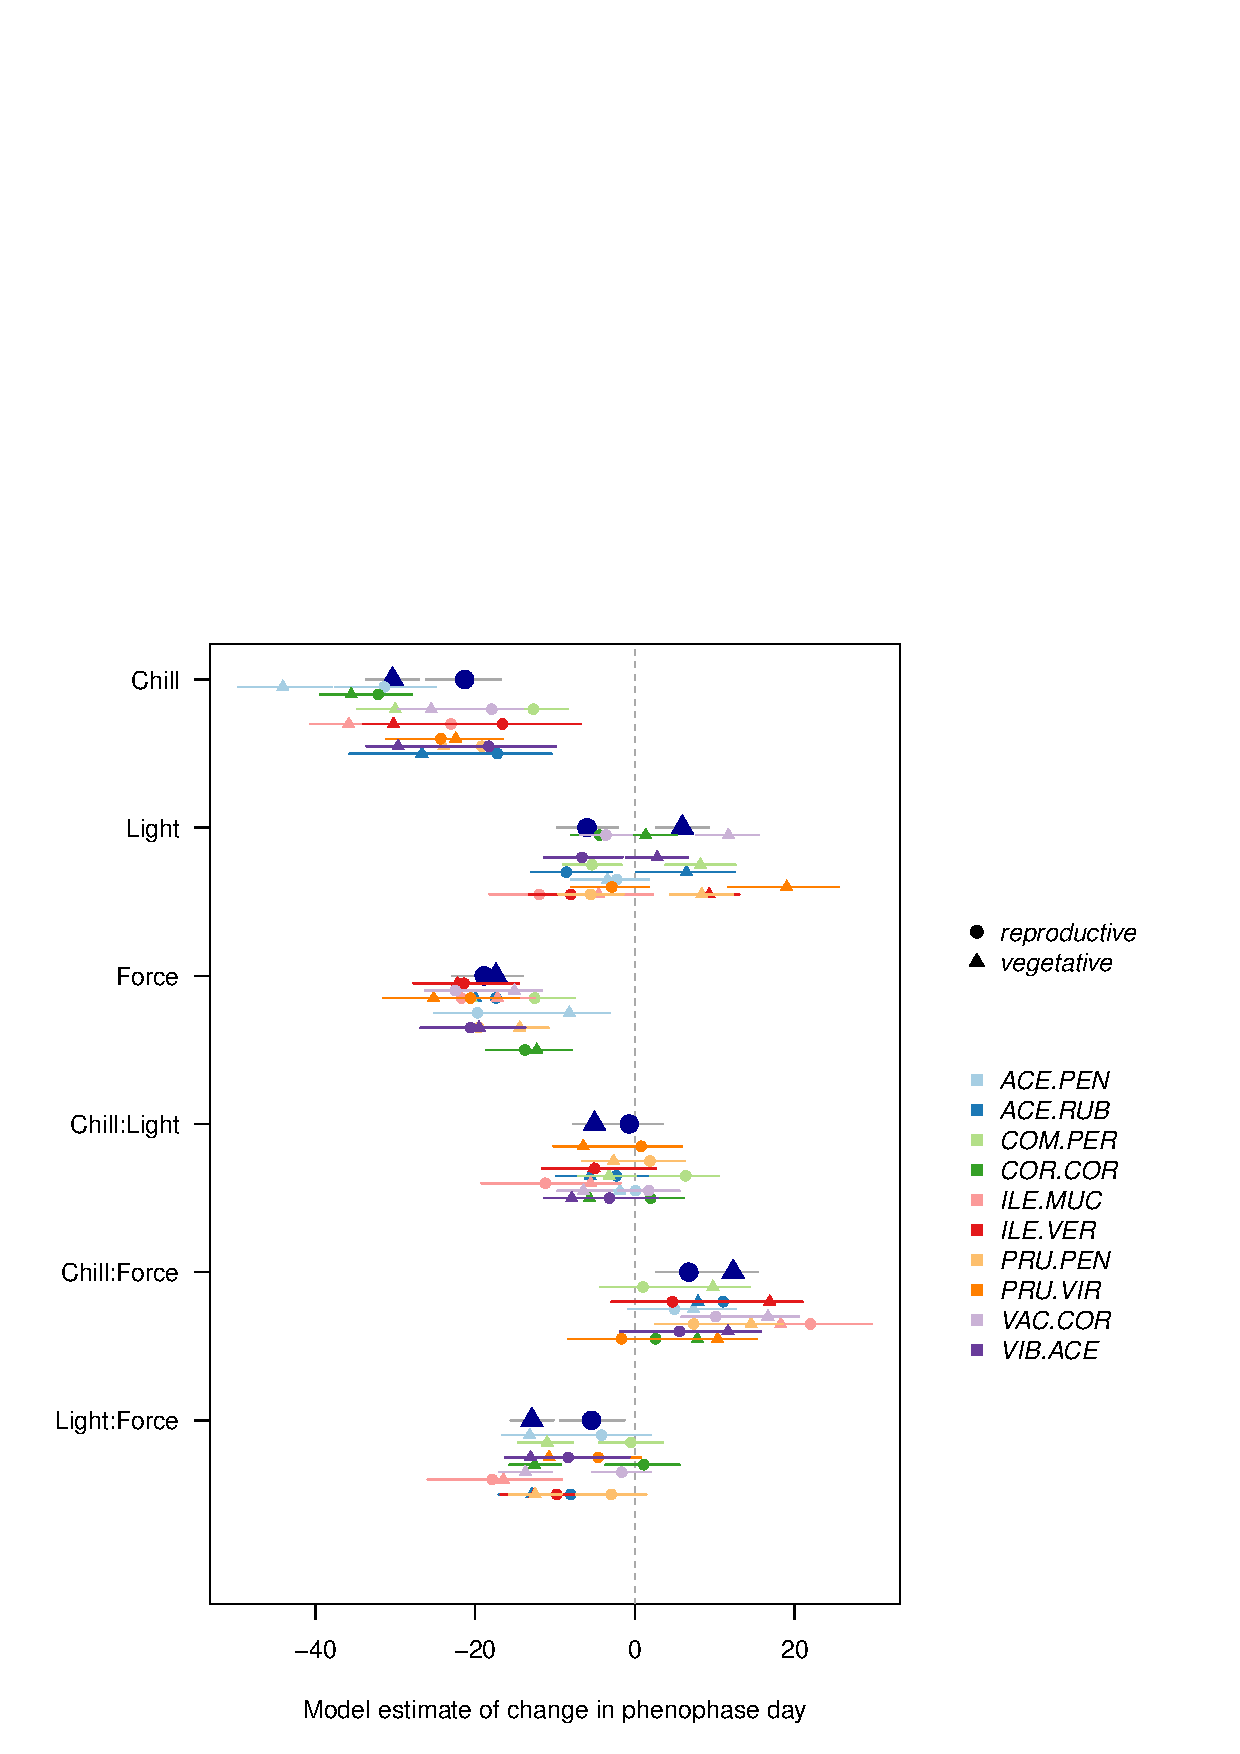
\includegraphics[width=\textwidth]{..//Plots/Flobuds_manuscript_figs/budburstvsflowering.pdf}
    \caption{\textbf{Experimental results suggest differential sensitivity to environmental cues between flower and leaf buds}. We used a growth chamber manipulation and Bayesian hierarchical models to evaluate the phenological sensitivity ($\Delta$ day of phenological event/ $\Delta$ environmental cue) of flower and leaf buds to varying forcing temperatures, photoperiods, and duration of chilling.   Vegetative buds (circles) were more sensitive to chilling and cue interactions. Flower buds (triangles) advanced with photoperiod increases under all treatment combinations but leaf phenology was delayed with increasing photoperiod when chilling and forcing levels were low. Points indicate mean estimates and lines represent the 50\% credible intervals. These differential sensitivities dictate how FLS patterns vary with changing environmental conditions.}
    \label{fig:model}
\end{figure}

\begin{figure}[h!]
    \centering
         \includegraphics[width=.8\textwidth]{..//Plots/Flobuds_manuscript_figs/phh_plot.png}
    \caption{\textbf{Under adequately long chilling duration and photoperiods, the phenological sensitivity ($\Delta$ phenological event/ $\Delta$ C$\degree$) follow the predicted pattern of the precocity hierarchy hypothesis (PHH), with the second phenophase of the sequence being approximately twice as sensitive to forcing as the first.} After performing a growth chamber manipulation evaluate the phenological sensitivity of flower and leaf buds to varying level forcing temperatures, photoperiods, and duration of chilling, we subset out data to include only observation at high chilling and photoperiod levels. Using Bayesian hierarchical models, we quantified the differences in sensitivity to forcing for all species in our study. Points indicate mean estimates and lines depict 50\% credible intervals. Our finding indications that the PHH should be considered a special case of the differential sensitivity hypothesis (DSH) that occurs when the chilling and photoperiod requirements are well met for both bud types.}
    \label{fig:phh}
\end{figure}

\pagebreak
%EMWOct2 -- I like the below one, I was going to suggest you keep the colors and put all on one panel, but I think this may work better as it stresses the wind versus biotic. I would just state more clearly in the caption that wind pollinated all leaf first -- that gets a little lost. 
\begin{figure}[h!]
    \centering
 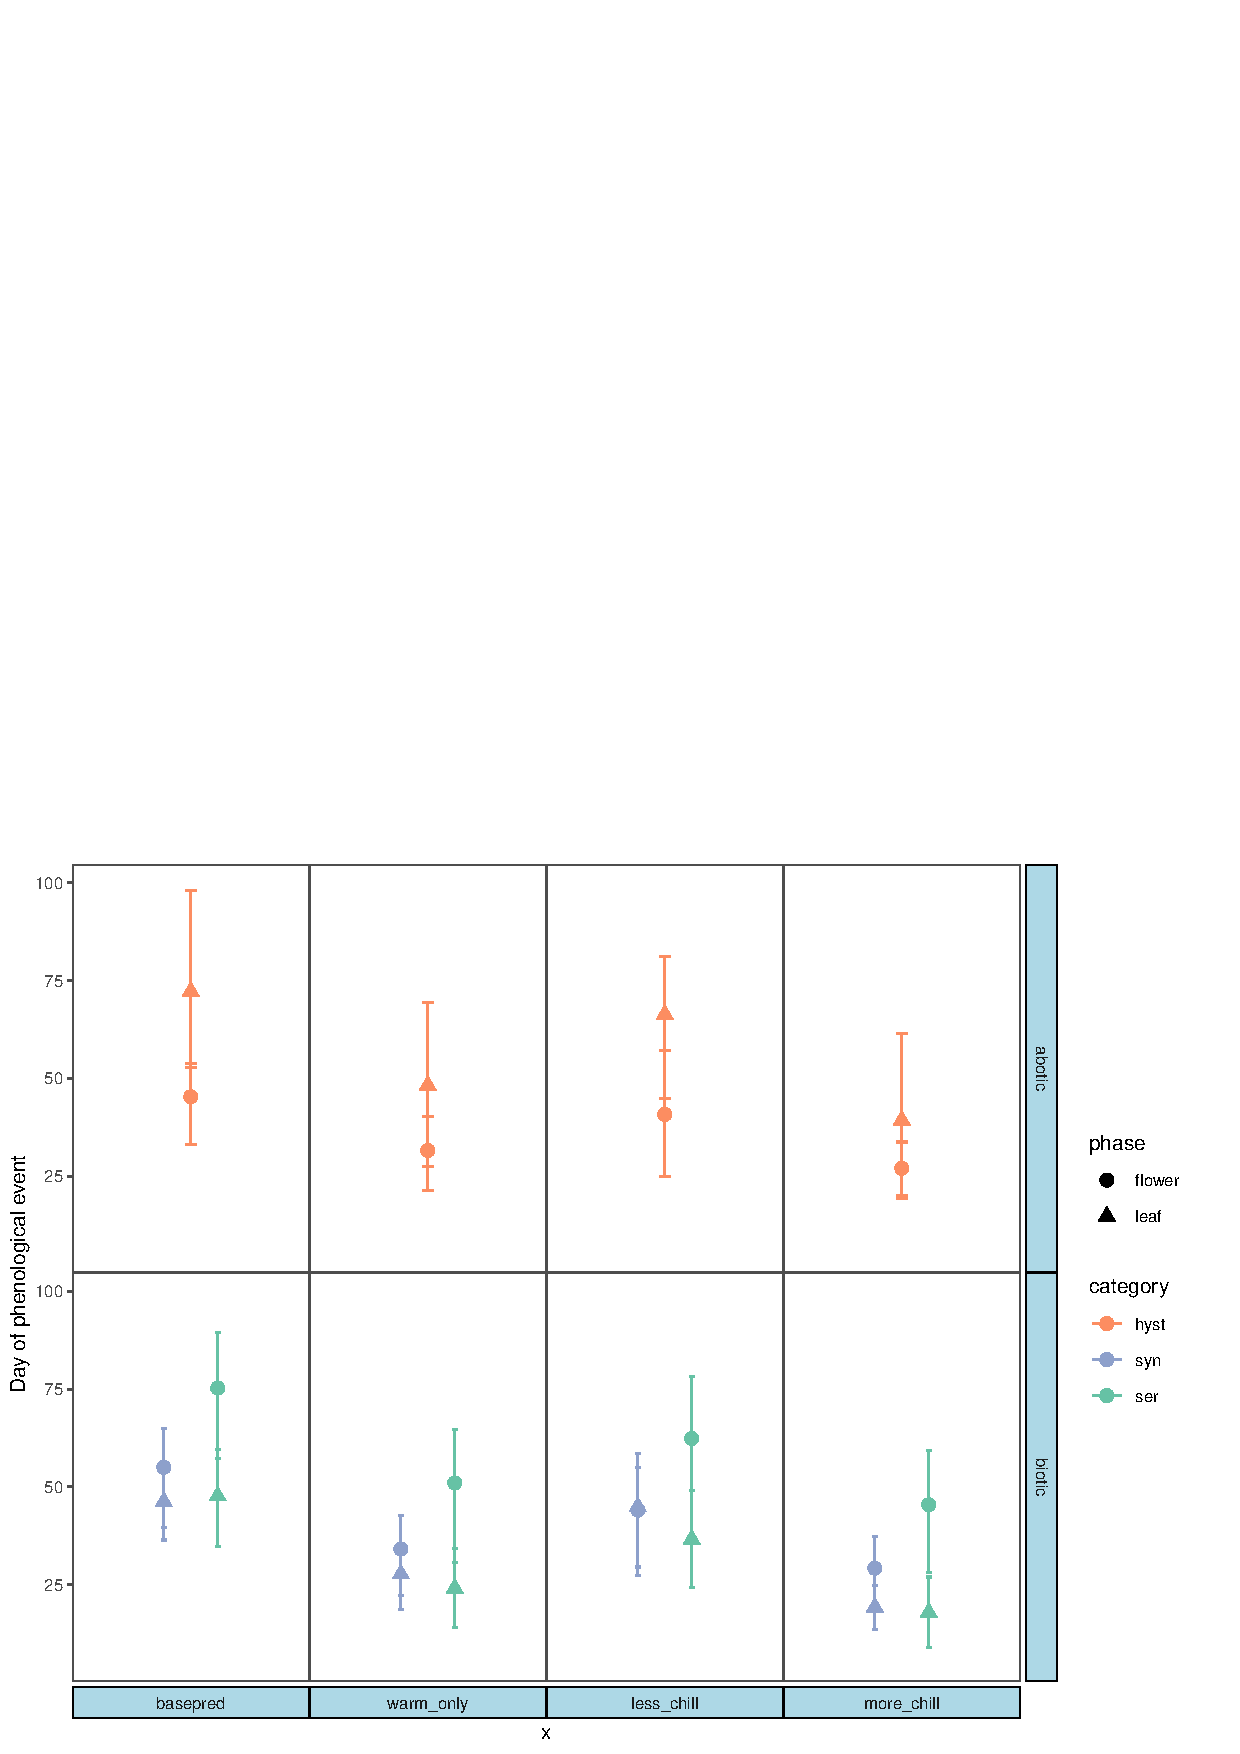
\includegraphics[width=.8\textwidth]{..//Plots/Flobuds_manuscript_figs/postergroups2.png}
    \caption{\textbf{Flower-leaf sequences (FLSs) of temperate, woody species will shift with climate change, but the magnitudes of these shifts vary by amonf FLS categories and depend on the specific dynamics of temperature at a given location.} We used Bayesian, hierarchical models comparing flower and leaf bud responses to variable temperature combinations to predict FLSs patterns under current climate conditions and three climate change scenarios;  an increase in spring warming alone (warm 5), increase in spring warming and increase in winter chilling (warm 5 +chill) and an increase in spring warming and decrease in winter chill (warm 5 -chill). We grouped the species-level posterior estimates by FLS category (flowering-first, concurrent, leafing-first). The points represent the mean estimates and the lines lines represent the 50\% credible intervals. Projected FLS shifts are most pronounced in wind-pollinated, flowering-first shrubs but FLS shifts for all species depend on the relationship between forcing and chilling changes which is likely to vary by location with climate change.}
    \label{fig:preddy}
\end{figure}


\begin{figure}[h!]
    \centering
 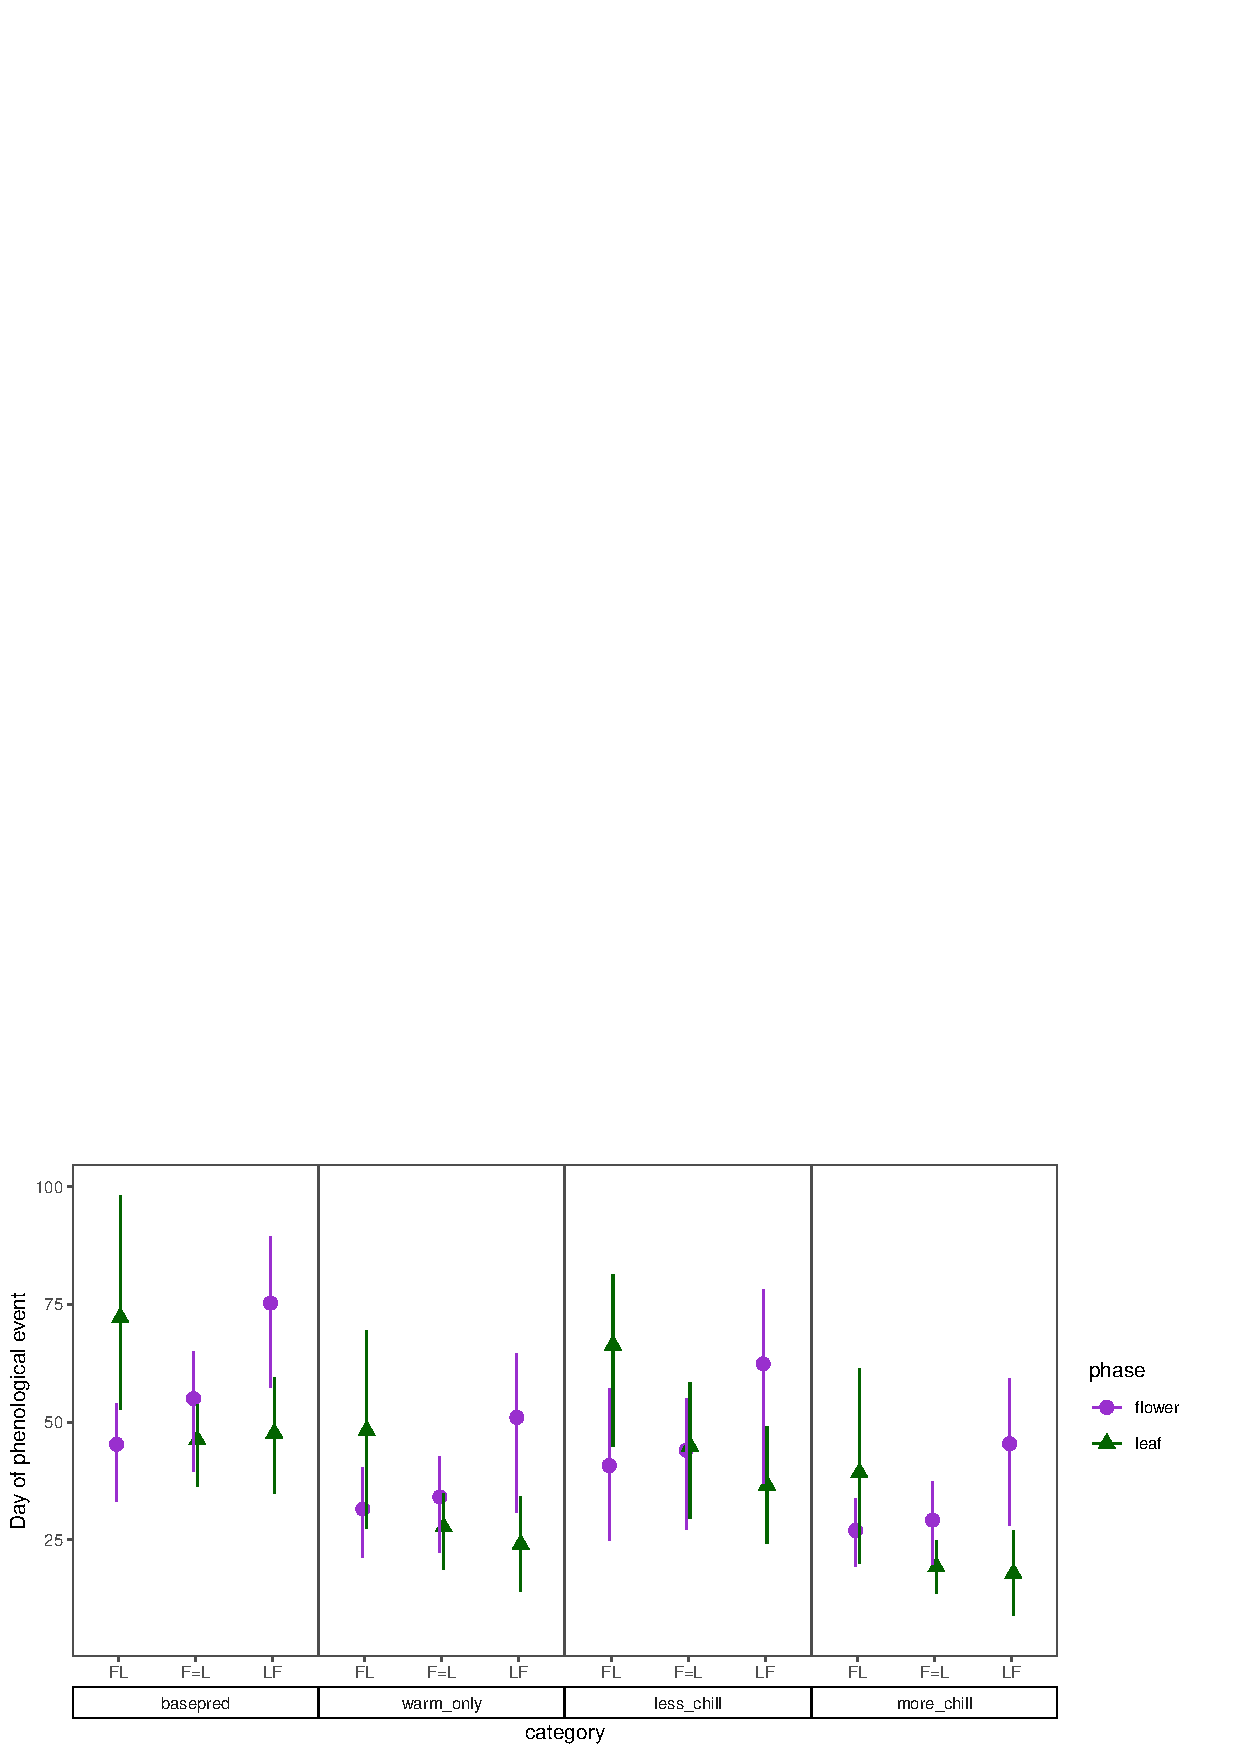
\includegraphics[width=\textwidth]{..//Plots/Flobuds_manuscript_figs/postergroups.png}
 \caption{Alternative Fig. \ref{fig:preddy}.}
 \end{figure}
%\subsection*{Differential sensitivity to environmental cues} %this is the old discussion
%\noindent The results of our experiment suggest that the relative timing of the component phases of flower-leaf sequences in deciduous, woody plants is structured by differences in the strength of the response of each bud type to the primary environmental cues of spring phenology. Specifically, vegetative buds were more sensitive to chilling and flower buds more sensitive to photoperiod. The sensitivity of flower and leaf buds to changes in forcing were proportionate in magnitude, but interactions between forcing and the other two cues drove a stronger response in leaf buds than flower buds. Together, the phenological response patterns we observed are more closely aligned with the predictions of the DSH than the PHH. Our results suggest that differential sensitivity to the environment among flower and leaf buds generates the high level of inter-annual FLS variation observed in nature, and will dictate the direction and magnitude of FLS shifts with climate change.\\.

%\noindent While both flower and leaf bud phenology advanced with increasing chilling duration, the sensitivity of the response to chilling was greater in leaf buds. This result is consistent with experimental manipulations of tree-crop phenology which also found a higher sensitivity to chilling for leaf buds \citep{Gariglio2006,Citadin2001}. We found that floral phenology was more tightly linked to changes in photoperiod than leaf phenology. While we found no literature that evaluated the differential sensitivity of flower and leaf buds to photoperiod, our findings are consistent with genetic work in the model genus \textit{Populus} suggests that flowering may be under stronger photoperiodic control that leafing \citep{}.\\

%\noindent Our results failed to support the PHH, but the patterns of phenological responses in our study may reveal key insights as to why this hypothesis may be so prevalent in the literature. We found that when we subset our data to include only high chilling and photoperiod treatments, the sensitivity of flower and leaf buds to forcing matched the predicted pattern of the PHH with the second phase of the phenological sequence demonstrating approximately twice the sensitivity of the first phase for many of these species of our studies (Fig. \ref{fig:phh}). This suggest that when chilling and photoperiod requirements are met, differences in the heat threshold requirements between flower and leaf buds structure FLSs.\\

%\noindent If under historic climate conditions the chilling requirement of most species was generally met in the field our results predict that the resulting FLS pattern would reflect a precocity hierarchy, and several of the studies that found support for the PHH are based on field observations \citep[e.g.][]{Guo2014,COSMULESCU:2020aa}. However, as winter temperature continue to change with global warming, it is likely that the regional chilling patterns will be disruption and the differential sensitivity of flower and leaf buds to the environment will have more pronounced effects on FLS patterns.

%\subsection*{FLS shifts with climate change}
%\noindent The support we found for the DSH in our study suggests that the direction and magnitude of FLS shifts with climate change will depend on how cues at a given location change relative to each other. We found that changes in the chilling cue strongly amplified the differential sensitivity of bud types to the environment, suggesting that this cue may drive FLS shifts with climate change. Because chilling only accumulates at intermediately low temperatures, warming may increase chilling at some locations while decreasing it in others \citep{}. This suggests that the direction and magnitude of FLS shifts is likely to vary substantially among populations based on the specific cue combinations at a given locality. Long-term phenology records show there was already substantial intra-specific variation in FLSs at the population level \citep{Buonaiuto2020} and our findings suggest that these populations level differences may be further amplified by climate change. There is currently little scholarship regarding how inter-population variation in FLS patterns may impact landscape processes like gene flow and dispersal, but given the hypothesized contribution of FLSs to reproductive fitness, this should remain an active area of research inquiry.\\

%\noindent Despite the fact that in our experiment we found photoperiod to be an important cue dictating FLS shifts, we modeled climate change scenarios with a constant photoperiod in our FLS projections with climate change. Climate change does not directly impact photoperiod, but warming does shift the time of year when plants become phenologically active, changing the photoperiod they experience. However, depending on the latitude, phenology would have to shifts by at minimum several weeks before the experience photoperiod would change substantially \citep{Ettinger}. However, at high latitudes where photoperiod changes more rapidly over the season, the experienced photoperiod may mute the FLS shifts captured in our projections. This may be particularly important as species shift shift their distribution pole ward with climate change and begin to encounter novel photoperiod regimes \citep{WAY:2015aa}.\\

%\noindent An additional complicating factor in predicting FLS shifts with climate change is that our experimental results and climate change projections suggest that species will differ in the direction and magnitude of their FLS shifts. Several species, \textit{Acer rubrum} ,\textit{Ilex verticillata}, \textit{Prunus pensylvanicum}, \textit{Prunus virginiana}, and \textit{Viburnum acerifolium}, had FLSs that were relatively robust to changing environments. For other species, \textit{Acer pensylvanicum}, \textit{Vaccinium corymbosum} and \textit{Ilex mucronata}, which typically begin to produce leaves shortly before flowers open, projected FLS shifts were moderate, with the combination of increased forcing coupled with a reduction in chilling driving the strongest shifts in FLSs. The two species with the most significant FLS shifts across treatment combinations and climate change projections were \textit{Comptonia peregrina} and \textit{Corylus cornuta} (Fig. \ref{fig:preddy}). In all of our climate change scenarios, the FLS interphase was dramatically reduced in these taxa.\\ 

%\noindent It is likely that these three difference response patterns we observed correlate to broader anatomical, physiological and phenological differences among species. We did not have the taxonomic resolution in this study to conclusively identify and character traits that may correlate with FLS shifts, but we observed some general patterns that may sever as starting hypotheses for future inquiry in this area.\\

%\noindent The species that maintained FLS structure across climate change scenarios generally shared a strongly leafing-first FLS, with a fairly long FLS interphase. These species tended to have mixed buds so there may be strong physical constraints on their FLSs. By contrast, the species that were most sensitive to FLS shifts were monoecious, flowering-first, wind-pollinated shrubs. This result may reflect other evidence that wind-pollinated species appear to be more sensitive to climate change than biotically pollinated taxa \citep{Ziello:2012aa}. Given the hypothesized function of FLS in wind-pollinated species, the direction and magnitude of FLS shifts we observed could suggest that that these species, and flowering-first, wind-pollinated taxa in general, may face particular risk for reproductive performance reductions. 

%\noindent Much of the conversation around phenology and pollination in the context of global change has centered around trophic mismatches between pollinator and floral phenology \citep{Memmott2007}, which is of little relevance to abiotically pollinated taxa. By contrast, the possibility that the effect of FLS shifts with climate change may be particularly important for abiotically pollinated woody plants and the scope and impact of FLS shifts in these taxa suggest they should be explored in greater detail in the future.\\

\end{document}